\documentclass[letter,12pt]{article}

\usepackage{ifpdf}
\makeatletter
\edef\texforht{TT\noexpand\fi
  \@ifpackageloaded{tex4ht}
    {\noexpand\iftrue}
    {\noexpand\iffalse}}
\makeatother
\ifpdf
  \usepackage[framemethod=TikZ]{mdframed}
\else
  \usepackage{framed}
  \def\pgfsysdriver{pgfsys-tex4ht-alt.def}
\fi

\title{PHYS 704 \\ Homework 10}
\author{Daniel Pad\'e}
\date{April 20, 2016}

\usepackage{enumerate}
\usepackage{amsfonts}
\usepackage{amsmath}
\usepackage{amssymb}
\usepackage{amsthm}
\usepackage{mathtools}
\usepackage{bm}
\usepackage{graphicx}
\usepackage{tikz}
\usepackage{float}
\usetikzlibrary{arrows}


\usepackage{fancyhdr}
\pagestyle{fancy}
\fancyhf{}
\fancyhead[LE,RO]{Daniel Pad\'e}
\fancyhead[RE,LO]{PHYS 704}
\fancyhead[CE,CO]{Homework 10}
\fancyfoot[LE,RO]{\thepage}

\theoremstyle{definition}
\newtheorem*{sol}{Solution}

\begin{document}
\newcommand{\bs}[1]{\boldsymbol{#1}}
\maketitle
\begin{enumerate}
    \item
        A flat right rectangular loop carrying a constant currint
        $I_1$ is placed near a long straight wire carrying a current
        $I_2$. The loop is oriented so that its center is a
        perpendicular distance d from the wire; the sides of length
        $a$ are parallel to the wire and the sides of length $b$ make
        an angle $\alpha$ with the plane containing the wire and the
        loop's center. The direction of the current $I_1$ is the same
        as that of $I_2$ in the side of the rectangle nearest the
        wire.
        \begin{enumerate}
            \item
                Show that the interaction magnetic energy
                \begin{align*}
                    W_{12} = \int \bs{J} \cdot \bs{A}_2 d^3x = I_1 F_2
                \end{align*}
                (where $F_2$ is the magnetic flux from $I_2$ linking
                the rectangular circuit carrying $I_1$), is
                \begin{align*}
                    W_{12} =
                    \frac{\mu_0 I_1 I_2 a} {4 \pi}
                    \ln
                    \left[
                        \frac
                        {4d^2 + b^2 + 4db \cos \alpha}
                        {4d^2 + b^2 - 4db \cos \alpha}
                    \right]
                \end{align*}
                \begin{sol}
                    \begin{align*}
                        W_{12} = I_1 \oint d\bs{l}_1 \cdot \bs{A}_2
                    \end{align*}
                    Take the loop to be in the x-y plane, centered at
                    the origin, with the wire above it as shown: \\
                    \begin{figure}[H]
                    \begin{tikzpicture}[x=0.25cm, y=0.25cm, z=0.15cm, >=stealth]
                        % The axes
                        \draw[dashed,arrows=->] (xyz cs:x=-5) -- (xyz cs:x=15) node[above] {$y$};
                        \draw[dashed,arrows=->] (xyz cs:y=0) -- (xyz cs:y=15) node[above] {$z$};
                        \draw[dashed,arrows=->] (xyz cs:z=5) -- (xyz cs:z=-15) node[above] {$x$};

                        % The loop
                        \draw[thick, -] (-5,0,5) -- (5,0,5);
                        \draw[thick, -] (-5,0,-5) -- (5,0,-5);

                        \draw[thick, -] (5,0,-5) -- (5,0,5);
                        \draw[thick, -] (-5,0,-5) -- (-5,0,5);

                        % Measurements
                        \draw[<->] (-5,0,6) -- (5,0,6);
                        \node at (0, 0, 7) {$a$};

                        \draw[<->] (-6,0,-5) -- (-6,0,5);
                        \node at (-7, 1, 0) {$b$};

                        \draw[<->] (0, 3, -2) -- (0, 0, 0);
                        \node at (2.5, 1.5, -2) {$d$};

                        % Wire
                        \draw[thick, <->] (-12, 3, -2) -- (12, 3, -2);

                        % currents
                        \draw[->] (-10, 3, 0) -- (-8, 3, 0);
                        \node at (-9, 4, 0) {$I_2$};

                    \end{tikzpicture}
                  \end{figure}
                    So $\bs{A}_2$ is given by
                    \begin{align*}
                        \bs{A}_2 = - \frac{I_2 \hat{\bs{y}}}{4 \pi}
                        \ln
                        \left[
                            {\left(
                                x - d \cos \alpha
                            \right)}^2
                            {\left(
                                x - d \sin \alpha
                            \right)}^2
                        \right]
                    \end{align*}
                    And only the sides of length $a$ will contribute:
                    \begin{align*}
                        \Rightarrow
                        W_{12} &= I_1 \oint d\bs{l}_1 \cdot \bs{A}_2
                        \\
                        &=
                        \frac{\mu_0 I_1 I_2 a}{4 \pi}
                        \ln
                        \left[
                            \frac
                            {{(-\frac{b}{2} - d \cos \alpha)}^2 - {(d \sin \alpha)}^2}
                            {{(\frac{b}{2} - d \cos \alpha)}^2 + {(d \sin \alpha)}^2}
                        \right]
                        \\
                        &=
                        \frac{\mu_0 I_1 I_2 a} {4 \pi}
                        \ln
                        \left[
                            \frac
                            {4d^2 + b^2 + 4db \cos \alpha}
                            {4d^2 + b^2 - 4db \cos \alpha}
                        \right]
                    \end{align*}
                \end{sol}
            \item
                Calculate the force between the loop and the wire for
                fixed currents.
                \begin{sol}
                    \begin{align*}
                        \bs{B} = \bs{\nabla} \times \bs{A}
                    \end{align*}
                    Only the force on the sides of length a will be nonzero by symmetry
                    \begin{align*}
                        B_x(x, 0) &=  - \frac{\partial A_y}{\partial z} \biggr \vert_{z=0}
                        \\
                        &=
                        \frac{-d \sin \alpha}
                        {{(x - d \cos \alpha)}^2 + {(d \sin \alpha)}^2}
                        \\
                        B_z(x, 0) &= \frac{\partial A_y}{\partial x} \biggr \vert_{z=0}
                        \\
                        &=
                        \frac{x-d \sin \alpha}
                        {{(x - d \cos \alpha)}^2 + {(d \sin \alpha)}^2}
                    \end{align*}
                    \begin{align*}
                        F_x &= I_1
                        \left[
                            B_z\left(\frac{b}{2}, 0\right) - B_z\left(-\frac{b}{2}, 0\right)
                        \right]
                        \\
                        &=
                        \frac{2 \mu_0 I_1 I_2 a b}{\pi}
                        \frac{4d^2 \cos(2\alpha) - b^2}
                        {b^4 - 8d^2\cos(2\alpha)b^2 + 16d^4}
                        \\
                        F_z &= - I_2
                        \left[
                            B_x\left(\frac{b}{2}, 0\right) - B_x\left(-\frac{b}{2}, 0\right)
                        \right]
                        \\
                        &=
                        \frac{8 \mu_0 I_1 I_2 a b}{\pi}
                        \frac{d^2 \sin(2\alpha)}
                        {b^4 - 8d^2\cos(2\alpha)b^2 + 16d^4}
                    \end{align*}
                \end{sol}
            \item
                Repeat the calculation for a circular loop of radius
                $a$, whose plane is parallel to the wire and makes an
                angle $\alpha$ with respect to the plane containing
                the center of the loop and the wire. Show that the
                interaction energy is
                \begin{align*}
                    W_{12} = \mu_0 I_1 I_2 d \cdot \Re
                    \left\{
                        e^{i\alpha} - \sqrt{e^{2i\alpha} - a^2 / d^2}
                    \right\}
                \end{align*}
                Find the force.
                \begin{sol}
                    Converting to cylindrical coordinates, $x = a\cos \phi$ and $dl_y = d\phi \; a \cos\phi$:
                    \begin{align*}
                        W_{12} = I_1 \int d\phi \; a \cos \phi A_y(a \cos \phi, 0)
                    \end{align*}
                    Expand $A_y$ in terms of $1/d$:
                    \begin{align*}
                        W_{12} = \mu_0 I_1I_2
                        \left(
                            \frac{a^2 \cos{\alpha}}{2d}
                            +
                            \frac{a^4 \cos(3\alpha)}{8d^3}
                            +
                            \cdots
                        \right)
                    \end{align*}
                    \begin{align*}
                        \frac{1 - \sqrt{1-z^2}}{z} = \frac{z}{2} + \frac{z^3}{8} + \cdots
                    \end{align*}
                    therefore
                    \begin{align*}
                        W_{12}
                        &= \mu_0 a I_1I_2
                        \Re\left(
                            \frac{1 - \sqrt{1 - {(\frac{a}{d}e^{i\alpha})}^2}}{\frac{a}{d}e^{i\alpha}}
                        \right)
                        \\
                        &= \mu_0 d I_1I_2
                        \Re\left(
                            e^{-i\alpha}
                            -
                            \sqrt{e^{-2i\alpha} - \frac{a^2}{d^2}}
                        \right)
                        \\
                        &= \mu_0 d I_1I_2
                        \Re\left(
                            e^{i\alpha}
                            -
                            \sqrt{e^{2i\alpha} - \frac{a^2}{d^2}}
                        \right)
                    \end{align*}
                    The last step is obtained from taking the real part.
                    \\
                    For the force, a similar process is applied to the following integral:
                    \begin{align*}
                        \bs{F} &= \hat{\bs{x}} I_1
                        \int d\phi\; a \cos \phi B_z(a \cos \phi, 0)
                        -
                        \hat{\bs{z}}I_1
                        \int d\phi\; a \cos \phi B_x(a \cos \phi, 0)
                    \end{align*}
                    yielding
                    \begin{align*}
                        F_x &= \mu_0 I_1 I_2
                        \Re\left[
                            \frac{1}{\sqrt{1 - \left(
                                \frac{a}{d}E^{i\alpha}
                            \right)}}
                        \right]
                        \\
                        F_z &= \mu_0 I_1 I_2
                        \Im\left[
                            \frac{1}{\sqrt{1 - \left(
                                \frac{a}{d}E^{i\alpha}
                            \right)}}
                        \right]
                    \end{align*}
                \end{sol}
            \item
                For both loops, show that when $d \gg a,b$ the
                interaction energy reduces to $W_{12} \approx \bs{m}
                \cdot \bs{B}$, where $\bs{m}$ is the magnetic moment
                of the loop. Explain the sign.
                \begin{sol}
                    \begin{align}
                        W_{12} &=
                        \frac{\mu_0 I_1 I_2 a} {4 \pi}
                        \ln
                        \left[
                            \frac
                            {4d^2 + b^2 + 4db \cos \alpha}
                            {4d^2 + b^2 - 4db \cos \alpha}
                        \right]
                        \\
                        &\approx
                        \frac{\mu_0I_1I_2a}{4\pi}
                        \frac{2b\cos(\alpha)}{d}
                        \\
                        &=
                        (I_1ab) \frac{\mu_0 I_2 \cos \alpha}{2 \pi d}
                        \\
                        &=
                        m_1 B_{2z}
                    \end{align}
                    Similarly for the second case:
                    \begin{align*}
                        W_{12} &\approx \mu_0 I_1 I_2 a \frac{a \cos \alpha}{2d}
                        \\
                        &=
                        (I_1 \pi a^2) \frac{\mu_0 I_2 \cos \alpha}{2 \pi d}
                        \\
                        &=
                        m_1 B_{2z}
                    \end{align*}
                    The sign is positive because the magnetic field
                    and the magnetic moment oppose each other.
                \end{sol}
        \end{enumerate}
    \item
        Show that the mutual inductance of two circular coaxial loops
        in a homogeneous medium of permeabililty $\mu$ is
        \begin{align*}
            M_{12} = \mu \sqrt{ab}
            \left[
                \left(
                    \frac{2}{k}
                    -
                    k
                \right)
                K(k)
                -
                \frac{2}{k}
                E(k)
            \right]
        \end{align*}
        where
        \begin{align*}
            k^2 =
            \frac{4ab}{(a + b^2) + d^2}
        \end{align*}
        and $a, b$ are the radii of the loops, $d$ is the distance
        between their centers, and $K$ and $E$ are the complete
        elliptic integrals.

        Find the limiting value when $d \ll a,b$ and $a \simeq b$
        \begin{sol}
          \begin{figure}[H]
            \begin{tikzpicture}[x=0.25cm, y=0.25cm, z=0.15cm, >=stealth]
                % The axes
                \draw[dashed,arrows=->] (xyz cs:x=-15) -- (xyz cs:x=15) node[above] {$y$};
                \draw[dashed,arrows=->] (xyz cs:y=-15) -- (xyz cs:y=15) node[above] {$z$};
                \draw[dashed,arrows=->] (xyz cs:z=15) -- (xyz cs:z=-15) node[above] {$x$};

                % ellipses
                \draw[thick] (0,10,0) ellipse (10 and 2);
                \draw[thick] (0,-10,0) ellipse (5 and 1);

                % radii
                \draw[->] (0, 10, 0) -- (10, 10, 0);
                \node at (5, 11, 0) {$a$};

                \draw[->] (0, -10, 0) -- (5, -10, 0);
                \node at (2.5, -8, 0) {$b$};

                % distance
                \draw[<->] (11, -10, 0) -- (11, 10, 0);
                \node at (9, 1, 0) {$d$};
            \end{tikzpicture}
          \end{figure}
            \begin{align*}
                M_{ij} &= \frac{1}{I_j} \int_{S_i} (\bs{\nabla} \times \bs{A}_{ij}) \cdot d\bs{a}
                \\
                &=
                \frac{1}{I_j}
                \oint_{C_i} \bs{A} \cdot d\bs{s_i}
                \\
                &=
                \frac{1}{I_j}
                \oint_{C_i}
                \left(
                    \frac{\mu I_j}{4 \pi}
                    \oint_{C_j} \frac{d\bs{s}_j}{r}
                \right)
                \cdot d\bs{s_i}
                \\
                &=
                \frac{\mu}{4 \pi} \oint_{C_i} \oint_{C_j} d\bs{s}_j \cdot d\bs{s}_i
            \end{align*}
            \begin{align*}
                d\bs{s}_1 &= a(-\hat{\bs{x}} \sin \phi_1 + \hat{\bs{y}}\cos\phi_1) d \phi_1
                \\
                d\bs{s}_2 &= b(-\hat{\bs{x}} \sin \phi_2 + \hat{\bs{y}}\cos\phi_2) d \phi_2
                \\
                \Rightarrow d\bs{s}_1 \cdot d\bs{s}_2 &=
                ab
                \left(
                    \sin \phi_1 \sin \phi_2 + \cos \phi_1 \cos \phi_2
                \right)
                d\phi_1 d\phi_2
                \\
                &= ab \cos (\phi_1 - \phi_2) d\phi_1 d\phi_2
            \end{align*}
            \begin{align*}
                r_1 &= a
                \left(
                    \hat{\bs{x}} \cos \phi_1
                    +
                    \hat{\bs{y}} \sin \phi_1
                \right)
                +
                \frac{d}{2}\hat{\bs{z}}
                \\
                r_2 &= b
                \left(
                    \hat{\bs{x}} \cos \phi_2
                    +
                    \hat{\bs{y}} \sin \phi_2
                \right)
                -
                \frac{d}{2}\hat{\bs{z}}
                \\
                r^2 = {(r_2 - r_1)}^2
                &=
                {\left[
                    (b \cos \phi_2 - a \cos \phi_1) \hat{\bs{x}}
                    +
                    (b \sin \phi_2 - a \sin \phi_1) \hat{\bs{y}}
                    -
                    d \hat{\bs{z}}
                \right]}^2
                \\
                &=
                a^2 + b^2 + d^2 - 2ab
                \left(
                    \cos \phi_1 \cos \phi_2 + \sin\phi_1 \sin\phi_2
                \right)
                \\
                &=
                a^2 + b^2 + d^2 - 2ab \cos(\phi_1 - \phi_2)
                \\
                \Rightarrow r &=
                \sqrt{a^2 + b^2 + d^2 - 2ab \cos(\phi_1 - \phi_2)}
            \end{align*}
            \begin{align*}
                M_{12} =
                \frac{\mu}{4 \pi}
                \oint_{\phi_2}
                d\phi_2
                \left(
                    \oint_{\phi_1}
                    d\phi_1\;
                    \frac
                    {ab\cos(\phi_1 - \phi_2)}
                    {\sqrt{a^2 + b^2 + d^2 - 2ab \cos(\phi_1 - \phi_2)}}
                \right)
            \end{align*}
            One of the integrals can be eliminated by performing the substitution
            $u = \phi_1 - \phi_2$, $du = d\phi_1$
            \begin{align*}
                M_{12} &=
                \frac{\mu}{4 \pi}
                \oint_{\phi_2}
                d\phi_2
                \left(
                    \oint_{u}
                    du\;
                    \frac
                    {ab\cos(u)}
                    {\sqrt{a^2 + b^2 + d^2 - 2ab \cos(u)}}
                \right)
                \\
                &=
                \frac{\mu}{4 \pi}
                \left(
                    \oint_{\phi_2}
                    d\phi_2
                \right)
                \left(
                    \oint_{u}
                    du\;
                    \frac
                    {ab\cos(u)}
                    {\sqrt{a^2 + b^2 + d^2 - 2ab \cos(u)}}
                \right)
                \\
                &=
                \frac{\mu}{2}
                \oint_{u}
                du\;
                \frac
                {ab\cos(u)}
                {\sqrt{a^2 + b^2 + d^2 - 2ab \cos(u)}}
            \end{align*}
            From a table:
            \begin{align*}
                \oint d\phi \frac{\cos \phi}{\sqrt{A - B \cos \phi}}
                &=
                \frac{4\sqrt{A + B}}{B}
                \left[
                    \left(
                        1 - \frac{k^2}{2}
                    \right)
                    K(k) - E(k)
                \right],
                & k = \sqrt{\frac{2B}{A + B}}
            \end{align*}
            Using the following substitutions:
            \begin{align*}
                A &\rightarrow \frac{a^2+b^2 +d^2}{a^2b^2}
                \\
                B &\rightarrow \frac{2}{ab}
                \\
                k &= \sqrt{
                \frac
                {4ab}
                {a^2 + b^2 + d^2 + 4}
                }
                \\
                M_{12} &= \mu
                \sqrt{a^2 + b^2 + d^2 + 4}
                \left[
                    \left(1 - \frac{k^2}{2}\right)K(k) - E(k)
                \right]
                \\
                &=
                \mu
                \frac{2\sqrt{ab}}{k}
                \left[
                    \left(1 - \frac{k^2}{2}\right)K(k) - E(k)
                \right]
                \\
                &=
                \mu
                \sqrt{ab}
                \left[
                    \left(\frac{2}{k} - k\right)K(k) - E(k)
                \right]
            \end{align*}
        \end{sol}
    \item
        A circular loop of mean radius $a$ is made of wire having a
        circular cross section of radius $b$, with $b \ll a$.  The
        sketch shows the relevant dimensions and coordinates for this
        problem.
        \begin{figure}[H]
        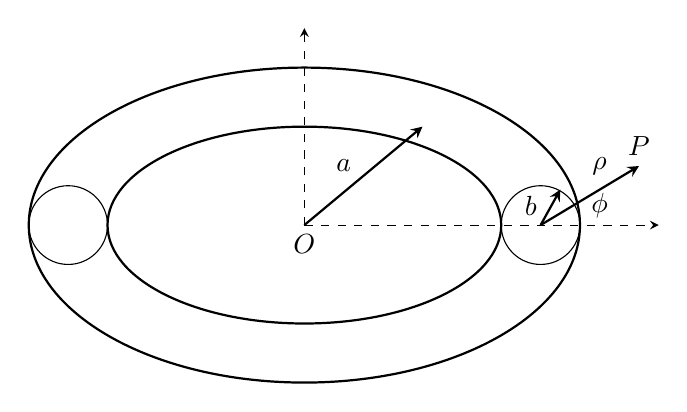
\begin{tikzpicture}[x=0.25cm, y=0.25cm, z=0.15cm, >=stealth]
            % The axes
            \draw[dashed,arrows=->] (xyz cs:x=0) -- (xyz cs:x=18);
            \draw[dashed,arrows=->] (xyz cs:y=0) node[below] {$O$} -- (xyz cs:y=10);

            % ellipses
            \draw[thick] (0,0,0) ellipse (10 and 5);
            \draw[thick] (0,0,0) ellipse (14 and 8);

            % main radius
            \draw[thick,->] (0, 0, 0) -- (6, 5, 0);
            \node at (2, 3, 0) {$a$};

            %% wire thickness
            \draw (12,0,0) circle [radius=2];
            \draw (-12,0,0) circle [radius=2];

            % dimensions
            \draw[thick, ->] (12, 0, 0) -- (13, 1.8, 0);
            \node at (11.5, 1, 0) {$b$};

            \draw[thick, ->] (12, 0, 0) -- (17, 3, 0) node[above] {$P$};
            \node at (15, 3, 0) {$\rho$};
            \node at (15, 1, 0) {$\phi$};
        \end{tikzpicture}
      \end{figure}
        \begin{enumerate}
            \item
                Using (5.37), the expression for the vector potential
                of a filamentary circular loop, and appropriate
                approximations for the elliptic integrals, show that
                the vector potential at the point $P$ near the wire is
                approximately
                \begin{align*}
                    A_\phi = (\mu_0 I / 2\pi) [\ln(8a / \rho) - 2]
                \end{align*}
                where $\rho$ is the transverse coordinate shown in the
                figure and corrections are of order $(\rho/a) \cos \phi$
                and ${(\rho / a)}^2$
                \begin{sol}
                    \begin{align*}
                        A_\phi(r, \theta)
                        =
                        \frac{\mu_0}{4\pi}
                        \frac{4Ia}{\sqrt{a^2 + r^2 + 2ar \sin \theta}}
                        \left[
                            \frac{(2-k^2)K(k) - 2E(k)}{k^2}
                        \right]
                    \end{align*}
                    where k is defined as
                    \begin{align*}
                        k^2 = \frac{4ar \sin \theta}{a^2 + r^2 + 2ar\sin\theta}
                    \end{align*}
                    \begin{align*}
                        r &= a + \rho \sin \phi
                        \\
                        \Rightarrow
                        a^2 + r^2 + 2ar \sin \theta
                        =
                        a^2 &+ {(a + \rho \sin \phi)}^2 + 2a(a + \rho \sin \phi)\sin \theta
                    \end{align*}
                    For $P$ close to the wire, $\sin \theta \approx 1$
                    \begin{align*}
                        \Rightarrow
                        a^2 + r^2 + 2ar \sin \theta
                        &=
                        a^2 + {(a + \rho \sin \phi)}^2 + 2a(a + \rho \sin \phi)
                        \\
                        &=
                        4a^2 + \rho^2 \sin^2 \phi + 4 a \rho \sin \phi
                    \end{align*}
                    \begin{align*}
                        k^2 &=
                        \frac{4a^2 + a\rho\sin\phi}
                        {4a^2 + \rho^2 \sin^2 \phi + 4 a \rho \sin \phi}
                        \\
                        &=
                        \frac{4 + \frac{\rho}{a} \sin \phi}
                        {4 + \frac{\rho^2}{a^2}\sin^2\phi + 4 \frac{\rho}{a}\sin\phi}
                        \\
                        &=
                        1 - 3 \frac{\rho}{4a} + \frac{\rho^2}{2a^2} + \mathcal{O}\left(\frac{\rho^3}{a^3}\right)
                    \end{align*}
                    \begin{align*}
                        A_\phi(r, \theta)
                        &=
                        \frac{\mu_0}{4\pi}
                        \frac{4Ia}{\sqrt{4a^2 + \rho^2 \sin^2 \phi + 4 a \rho \sin \phi}}
                        \left[
                            \frac{(2 - k^2)K(k) - 2E(k)}{k^2}
                        \right]
                        \\
                        &=
                        \frac{\mu_0}{4\pi}
                        \frac{4I}
                        {\sqrt{4 + \frac{\rho^2}{a^2} \sin^2 \phi + 4 \frac{\rho}{a} \sin \phi}}
                        \left[
                            \frac{(1 + \frac{3\rho}{4a})K(k) - 2E(k)}{1 - \frac{3\rho}{4a}}
                        \right]
                    \end{align*}
                    \begin{align*}
                        K(k) = \int_0^{\frac{\pi}{2}}
                        \frac{d\theta}{\sqrt{1 - k^2 \sin^2 \theta}}
                        &=
                        \frac{\pi}{2}
                        \left\{
                            1 + \frac{1}{4}\left(1 - \frac{3 \rho}{4 a}\right)
                        \right\}
                        \\
                        &=
                        \frac{\pi}{8}
                        \left(
                            5 - \frac{3\rho}{4a}
                        \right)
                        \\
                        E(k) = \int_0^{\frac{\pi}{2}}
                        d\theta\;\sqrt{1 - k^2 \sin^2 \theta}
                        &=
                        \frac{\pi}{2}
                        \left\{
                            1 - \frac{1}{4}\left(1 - \frac{3 \rho}{4 a}\right)
                        \right\}
                        \\
                        &=
                        \frac{3\pi}{8}
                        \left(
                            1 + \frac{\rho}{4a}
                        \right)
                    \end{align*}
                    \begin{align*}
                        A_\phi(r, \theta)
                        &=
                        \frac{\mu_0}{4\pi}
                        \frac{4I}
                        {\sqrt{4 + \frac{\rho^2}{a^2} \sin^2 \phi + 4 \frac{\rho}{a} \sin \phi}}
                        \left[
                            \frac{\pi}{8}
                            \frac{(1 + \frac{3\rho}{4a})
                            (5 - 3\rho / 4 a) - 2(3 + 3\rho / 4a)}{1 - \frac{3\rho}{4a}}
                        \right]
                        \\
                        &=
                        \frac{\mu_0 I}{8}
                        \left(
                            \frac{1}{2}
                            -
                            \frac{1}{4}\frac{\rho}{a}\sin \phi
                        \right)
                        \left[
                            \frac{(1 + \frac{3\rho}{4a})
                            (5 - 3\rho / 4 a) - 2(3 + 3\rho / 4a)}{1 - \frac{3\rho}{4a}}
                        \right]
                        \\
                        &=
                        \frac{\mu_0 I}{8}
                        \left(
                            \frac{1}{2}
                            -
                            \frac{1}{4}\frac{\rho}{a}\sin \phi
                        \right)
                        \left[
                            \frac{-1 + 21 \rho / 4 a}{1 - \frac{3\rho}{4a}}
                        \right]
                        \\
                        &=
                        \frac{\mu_0 I}{8}
                        \left(
                            \frac{1}{2}
                            -
                            \frac{1}{4}\frac{\rho}{a}\sin \phi
                        \right)
                        \left[
                            \frac{-1 + 21 \rho / 4 a}{1 - \frac{3\rho}{4a}}
                        \right]
                        \\
                        &= \cdots
                    \end{align*}
                \end{sol}
            \item
                Since the vector potential of part a is, apart from a
                constant, just that outside a straight circular wire
                carrying a current $I$, determine the vector potential
                inside the wire $(\rho < b)$ in the same approximation
                by requiring continuity of $A_\phi$ and its radial
                derivative at $\rho = b$, assuming that the current is
                uniform in density inside the wire:
                \begin{align*}
                    A_\phi &=
                    (\mu_0 I / 4 \pi)(1 - \rho^2 / b^2)
                    +
                    (\mu_0 I / 2 \pi)
                    [\ln(8a / b) - 2],
                    &
                    \rho < b
                \end{align*}
            \item
                Use (5.149) to find the magnetic energy, hence the
                self-inductance,
                \begin{align*}
                    L = \mu_0a[\ln(8a/b) - 7/4]
                \end{align*}
                Are the corrections of order $b/a$ or ${(b/a)}^2$?
                What is the change in $L$ if the current is assumed to
                flow only on the surface of the wire (as occurs at
                high frequencies when the skin depth is small compared
                to $b$)?
        \end{enumerate}
\end{enumerate}
\end{document}
